
%----------------------------------------------------------------------------------------
%	Lecture 20
%----------------------------------------------------------------------------------------

\chapter{Simply Connected Region}

\bigbreak

\section{Green's Theorem With Singularity}

We know that Green's theorem is defined only if $curl({\bf F})$ is defined everywhere inside the region.
For example, 
$$
{\bf F} = \frac{\ij{-y}{x}}{x^2 + y^2}
$$

This vector field is not defined at the origin and the $curl({\bf F}) = 0$ because
\begin{align*}
    curl({\bf F}) & = N_x - M_y \\
    & = \px{}{x} \frac{x}{x^2+y^2} - \px{}{y} \frac{-y}{x^2+y^2} \\
    & = \frac{1}{x^2 + y^2} + \frac{- x * 2x}{(x^2 + y^2)^2} + \frac{1}{x^2 + y^2} + \frac{- y * 2 y}{(x^2 + y^2)^2} \\
    & = \frac{y^2 - x^2}{(x^2 + y^2)^2} + \frac{x^2 - y^2}{(x^2 + y^2)^2} \\
    curl({\bf F}) & = 0
\end{align*}

So any line integral over a closed loop should be zero by Green's Theorem if the region does not contain the origin.
But what happens at origin? Let's take a circle of radius $a$ centered at origin. Note that we cannot use Green's theorem to evalute this integral.
So,

$$
\oint_C {\bf F} \cdot d{\bf r} = \oint_C Mdx + Ndy = \oint_C \frac{-y}{x^2 + y^2} dx + \frac{x}{x^2 + y^2} dy
$$

Since, it is a circle we can parametrize as $x = a \cos \theta$ and $y = a \sin \theta$ and $x^2 + y^2 = a^2$.
Thus, we get $dx = - a \sin \theta d\theta$ and $dy = a \cos \theta d\theta$.
And the limits of $\theta$ are  $0$ to $2\pi$.
So, our integral becomes, 
\begin{align*}
\oint_C {\bf F} \cdot d{\bf r} & = \int_0^{2\pi} \frac{- a \sin \theta}{a^2} (- a \sin \theta d\theta) + \frac{a \cos \theta}{a^2} (a \cos \theta d\theta) \\
& = \int_0^{2\pi} (\sin^2 \theta + \cos^2 \theta) d\theta = \int_0^{2\pi} 1 d\theta = 2 \pi
\end{align*}

Thus, we've shown that since the vector field ${\bf F}$ is not defined at the origin so the closed loop containing the origin does not follow Green's Theorem.

\pagebreak

\section{Excluding The Singularity}

We claim that if we take two curves $C1 = ABCDA$ and $C2 = EFGHE$ both going clockwise as show below.
Then the difference of their line integrals will follow Green's Theorem.

{\bf Note: } The curves can be anyshape as long as the both contain the singularity individually and the region between them does not conatin any singularity.

\begin{figure}[ht!]
    \centering
    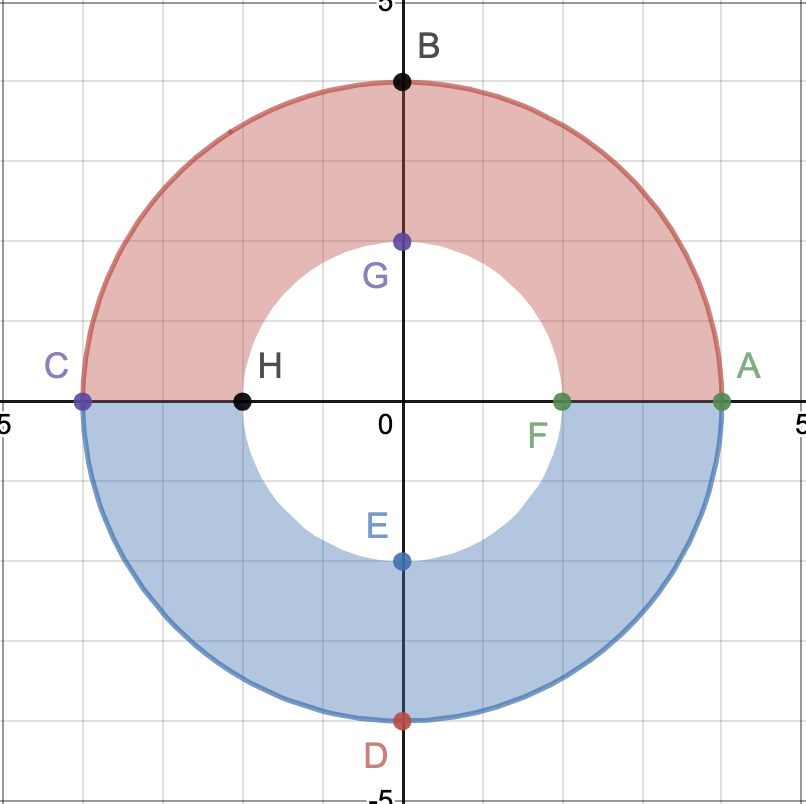
\includegraphics[scale=0.5]{./images/lecture_20_figure_1.png}
    \caption{Two Circles centered at origin}
\end{figure}

That is, 
$$
\int_{C_1} {\bf F} \cdot d{\bf r} - \int_{C_2} {\bf F} \cdot d{\bf r} = \iint_R curl({\bf F}) dA
$$

We can prove this by dividing the region into two separate closed regions : $ABCHGFA$ (colored red) and $ADCHEFA$ (colored blue).
${\bf F}$ is defined on both of these regions so we can apply Green's Theorem and we get the above formula.
The line integral along the lines $CH$ and $AF$ cancel out as we integral along them twice in opposite directions.

We can check this for the example given in last section.
The difference of line integrals will be zero as it is a constant for concentric circles.
And the double integral will be zero as the curl is zero.

\section{Simply Connected Region}

{\bf Definition : } A region $R$ is simply connected if the interior of any closed curve in $R$ is also contained in $R$.

This guarantees that if a vector field is defined and differentiable inside a simply connected region then it will be defined and differentiable for any region bound by a closed curve 
in the simply connected region.

In the example above, the vector field is not defined at the origin so the XY-plane with the origin removed is not simply connected.


{\bf Corollary : } If $curl({\bf F}) = 0$ and the domain of region where ${\bf F}$ is defined and differentiable is simply connected then ${\bf F}$ is conservative and ${\bf F}$ is a gradient field.